\documentclass[twoside=false, %  doppelseitiger Druck
    DIV=12,% DIV Faktor für Satzspiegelberechnung, sie Doku zu KOMA Script
%    BCOR=15mm, % Bindekorrektur
    chapterprefix=false,
    headinclude=true,
    footinclude=false,
    mpinclude=false,
    pagesize,%         write pagesize to DVI or PDF
    fontsize=11pt,%             use this font size
    paper=a4,%          use ISO A4
    bibliography=totoc,%         write bibliography-chapter to table of contents
    index=totoc,%         write index-chapter to table of contents
    cleardoublepage=plain,% \cleardoublepage generates pages with pagestyle empty
    headings=big,%       A4/B5
    listof=flat,%        improved list of tables
    numbers=noenddot
  ]{scrbook}

\usepackage{scrhack}
\usepackage[utf8]{inputenc}
\usepackage{makeidx}
\usepackage{amsfonts}
\usepackage[slantedGreek,sc]{mathpazo}  % Schriftart Palatino
%\usepackage{lmodern}    % statt mathpazo, falls CM Fonts verwendet werden sollen
%\usepackage{mathptmx}    % statt mathpazo, falls Times  verwendet werden soll
\usepackage[scaled=.95]{helvet}
\usepackage{courier}
\usepackage[T1]{fontenc}
\usepackage{textcomp}
\usepackage{amsmath}            % standard math notation (vectors/sets/...)
\usepackage{bm}        % standard math notation (fonts)
\usepackage{fixmath}        % standard math notation (fonts)
\usepackage{graphicx}
\usepackage[facing=yes]{floatrow}       % mehrere Gleitobjekte nebeneinander/caption neben Bild/Tabelle
\usepackage[labelfont=bf,sf,font=small,labelsep=space,format=plain]{caption}
\usepackage{subcaption}
\usepackage{scrpage2}
% \usepackage{pstool}  % einbinden falls psfrag verwendet werden soll
\usepackage{epstopdf}
\usepackage[ngerman]{babel}
\usepackage{csquotes}
\usepackage{ellipsis}  % Korrigiert den Weißraum um Auslassungspunkte
\usepackage{microtype}  % optischer Randausgleich etc.
\usepackage{url}
\usepackage[backend=bibtex,style=alphabetic]{biblatex}
% temorary fix: siehe auch -->
%http://tex.stackexchange.com/questions/311426/bibliography-error-use-of-blxbblverbaddi-doesnt-match-its-definition-ve
\makeatletter
\def\blx@maxline{77}
\makeatother

\usepackage[table,dvipsnames]{xcolor}         % z.B. für schattierte Boxen
\usepackage{framed}			% shaded Umgebung
\usepackage[printonlyused]{acronym}
\usepackage{tabulary}
\usepackage{tabularx}
% \usepackage{booktabs}
\usepackage{ifthen}
 \usepackage{float}
\usepackage{pifont}
\usepackage{marginnote}
\usepackage[strict]{changepage}
\usepackage{longtable,array,ragged2e,multirow}
% Links im PDF
\usepackage[colorlinks=false,pdfborder={0 0 0},breaklinks=true]{hyperref}
\usepackage{tcolorbox}
\usepackage{listings}
\usepackage{upquote}
\usepackage{todonotes}
\usepackage{sourcecodepro}

\tcbuselibrary{skins}

\pdfoptionpdfminorversion=7

%---------------- colors ------------------%
\definecolor{primary}{HTML}{1A71B3}%
\definecolor{secondary}{HTML}{283593}%
\definecolor{accent}{HTML}{FF9800}%
\colorlet{background}{primary!20}%

%Code
\definecolor{strings}{HTML}{008000} % for strings
\definecolor{comments}{rgb}{0.25,0.5,0.35} % comments
%\colorlet{keywords}{primary} % keywords
\definecolor{keywords}{HTML}{000080} % keywords
\definecolor{ndkeywords}{HTML}{660E7A} % keywords
\definecolor{javadoc}{rgb}{0.25,0.35,0.75} % javadoc
\definecolor{codebackground}{HTML}{F8F8F8} %
\colorlet{codeborder}{gray} %
%-------------- end colors ----------------%

%-------------- lengths ----------------%
\newlength{\twfivec} %tablewidth für 5 Spalten
\setlength{\twfivec}{\textwidth} %setze neue länge auf textbreite
\addtolength{\twfivec}{-10\tabcolsep} %5 Spalten
%------------- end lengths ---------------%

%------------- customizations -------------%
\makeindex

\recalctypearea

\selectlanguage{ngerman}

\setkomafont{paragraph}{\normalfont\normalsize\bfseries}

\deffootnote{1em}{1em}{\makebox[1em][l]{\thefootnotemark}}

% Einstellungen für Bild-/Tabellenbeschriftung neben dem Bild
\floatsetup[figure]{capbesideposition={inside,top}}
\floatsetup[table]{capbesideposition={inside,top},style=plaintop}
\renewfloatcommand{fcapside}{figure}[\capbeside][\FBwidth]
\newfloatcommand{tcapside}{table}[\capbeside][\FBwidth]

\newcolumntype{L}[1]{>{\RaggedRight\arraybackslash}p{#1}}
\newcolumntype{C}[1]{>{\centering\arraybackslash}p{#1}}

\lstdefinelanguage{TypeScript}{
  keywords={typeof, new, true, false, catch, function, return, null, catch, switch, var, if, in, while, do, else, case, break, class, export, boolean, throw, implements, import, from, this},
  ndkeywords={selector, template, styles},
  sensitive=false,
  comment=[l]{//},
  morecomment=[s]{/*}{*/},
  showstringspaces=false,
  morestring=[b]',
  morestring=[b]",
  morestring=[b]`
}

\lstdefinestyle{typescript}{
  language=TypeScript,
  basicstyle=\ttfamily,
  keywordstyle=\color{keywords}\bfseries,
  ndkeywordstyle=\color{ndkeywords}\bfseries,
  identifierstyle=\color{black},
  commentstyle=\color{comments}\ttfamily,
  stringstyle=\color{strings}\bfseries,
  literate={`}{{\`{}}}1
  %  numbers=left,
  %  numberstyle=\tiny\color{black},
  %  stepnumber=1,
  %  numbersep=10pt,
}

\lstset{basicstyle=\ttfamily}

\newtcolorbox{borderbox}[2][]{
	colback=background,
	colframe=primary,
	sharp corners=all,
	boxrule=1pt,
	fonttitle=\bfseries,
	left=12pt,
	enlarge top by=1em,
  	enlarge bottom by=1em,
	title=#2,
	#1
}

\newtcolorbox{codebox}{
	colback=codebackground,
	colframe=codeborder,
	sharp corners=all,
	boxrule=0.5pt,
	left=2em,
	top=0em,
	bottom=0em,
	enlarge top by=.5em,
  	enlarge bottom by=.5em,
}

\newtcolorbox{simplebox}[1][]{
	colback=background,
	colframe=primary,
	sharp corners=all,
	fonttitle=\bfseries,
	toprule=0pt,
	leftrule=2pt,
	rightrule=0pt,
	bottomrule=0pt,
	#1
}
%------------- end customizations -------------%

%----------------  renew commands ------------------%
\renewcommand{\marginfont}{\strut\hskip-1em % Das ist erst einmal ein
                                % gemeiner Trick zur korrekten Ausrichtung
                                % kleiner Fontgrößen mit abweichendem
                                % Zeilenabstand.
  \linespread{1}\footnotesize% Das ist der Rest.
}
\renewcommand{\marginfont}{\footnotesize}

\renewcommand{\thempfootnote}{\arabic{mpfootnote}}
%--------------  end renew commands ----------------%

%--------------- new commands ----------------------%
\newcommand{\real}{\mathord{\mathrm{I\!R}}}

\newcommand{\acr}[1]{\acs{#1} (\aclu{#1})}
\newcommand{\acrp}[1]{\acsp{#1} (\aclp{#1})\acused{#1}}
%---------------- end new commands ----------------%

%--------------- new environments ----------------------%
%deprecated, use simplebox istead
\newenvironment{citeenv}{%
  \def\FrameCommand{%
    \hspace{1pt}%
    {\color{primary}\vrule width 2pt}%
    {\color{background}\vrule width 1em}%
    \colorbox{background}%
  }%
  \MakeFramed{\advance\hsize-\width\FrameRestore}%
  % \noindent\hspace{-4.55pt}% disable indenting first paragraph
  \begin{adjustwidth}{}{7pt}%
  \vspace{.5em}%
}
{%
  \vspace{.5em}\end{adjustwidth}\endMakeFramed%
}
%--------------- end environments ----------------------%

\addbibresource{thesis.bib}

%=============== beginn document ======================%
\begin{document}
\selectlanguage{ngerman}
\def\figdir{figures}
\def\tabledir{tables}

\frontmatter
\pagenumbering{alph}
\pagestyle{scrplain}
\pagestyle{empty}

\begin{titlepage}

\sffamily

\raggedleft


\includegraphics{\figdir/HS_Logo_aktuell_CMYK.eps}

\vfill

\centering
\Large
% \vspace*{\fill}
%-----------
Hochschule Rosenheim\\
Fakultät für Informatik
\vspace{2cm}\\
%-----------
 \Large
Studienarbeit\vspace{1cm}\\
%-----------
 \Large
 Sofware-Architektur WS 2016/17 \\
 \Large
%-----------

\vspace*{\fill}

Michael Hutterer

Martin Neumayer

Marcel Pütz

Franz Wimmer 

\vspace{1cm}

 \LARGE

Offline First with PouchDB and Angular 2
\vspace{1cm}

\flushleft
 \Large
\vspace*{\fill}

%-----------
\begin{tabbing}
\hspace*{4cm}\= \kill
Lehrbeauftragter:\> Stefan Frai\\
Verantwortlich:\> Prof.\ Dr.\ Gerd Beneken\\
\end{tabbing}
%-----------

\end{titlepage}

\cleardoubleemptypage

{
\large
\thispagestyle{empty}
\vspace*{\fill}

\noindent
\textsc{Erklärung}

\medskip

\noindent
Wir versicheren, dass wir diese Arbeit selbständig
angefertigt, nicht anderweitig für Prüfungszwecke
vorgelegt, keine anderen als die angegebenen Quellen
oder Hilfsmittel benützt sowie wörtliche und
sinngemäße Zitate als solche gekennzeichnet haben.

\bigskip

\noindent
Rosenheim, den \today

\vspace*{2cm}

\noindent
 Michael Hutterer\hspace{.8cm} Martin Neumayer \hspace{.8cm} Marcel Pütz \hspace{.8cm} Franz Wimmer\\
}

%%% Local Variables:
%%% mode: latex
%%% TeX-master: "d"
%%% End:

\cleardoubleemptypage

\pagestyle{scrplain}
\pagenumbering{roman}
% ---------------------------------------------------
% D-TOC.TEX zur Verwendung mit TEXPART
% (an eigene Gegebenheiten anzupassen)
% ---------------------------------------------------
%
\tableofcontents
\clearpage
\listoffigures
\cleardoublepage


\pagestyle{scrheadings}


\addtokomafont{caption}{\small}

\mainmatter

\chapter{Einleitung und Zielsetzung}
\label{chap:Einleitung und Zielsetzung}
\section{Coole Einleitung}
\label{sec:Coole Einleitung}
Lorem ipsum dolor sit amet, consetetur sadipscing elitr, sed diam nonumy eirmod tempor invidunt ut labore et dolore magna aliquyam erat, sed diam voluptua. At vero eos et accusam et justo duo dolores et ea rebum. Stet clita kasd gubergren, no sea takimata sanctus est Lorem ipsum dolor sit amet. Lorem ipsum dolor sit amet, consetetur sadipscing elitr, sed diam nonumy eirmod tempor invidunt ut labore et dolore magna aliquyam erat, sed diam voluptua. At vero eos et accusam et justo duo dolores et ea rebum. Stet clita kasd gubergren, no sea takimata sanctus est Lorem ipsum dolor sit amet. Lorem ipsum dolor sit amet, consetetur sadipscing elitr, sed diam nonumy eirmod tempor invidunt ut labore et dolore magna aliquyam erat, sed diam voluptua. At vero eos et accusam et justo duo dolores et ea rebum. Stet clita kasd gubergren, no sea takimata sanctus est Lorem ipsum dolor sit amet.

Duis autem vel eum iriure dolor in hendrerit in vulputate velit esse molestie consequat, vel illum dolore eu feugiat nulla facilisis at vero eros et accumsan et iusto odio dignissim qui blandit praesent luptatum zzril delenit augue duis dolore te feugait nulla facilisi. Lorem ipsum dolor sit amet, consectetuer adipiscing elit, sed diam nonummy nibh euismod tincidunt ut laoreet dolore magna aliquam erat volutpat.

Eine Abbildung referenziert man so: Abbildung \ref{fig:bsp}

\begin{figure}[ht]
\centering
\caption{Hier ein Beispiel für das Einbinden einer Grafik}
\label{fig:bsp}
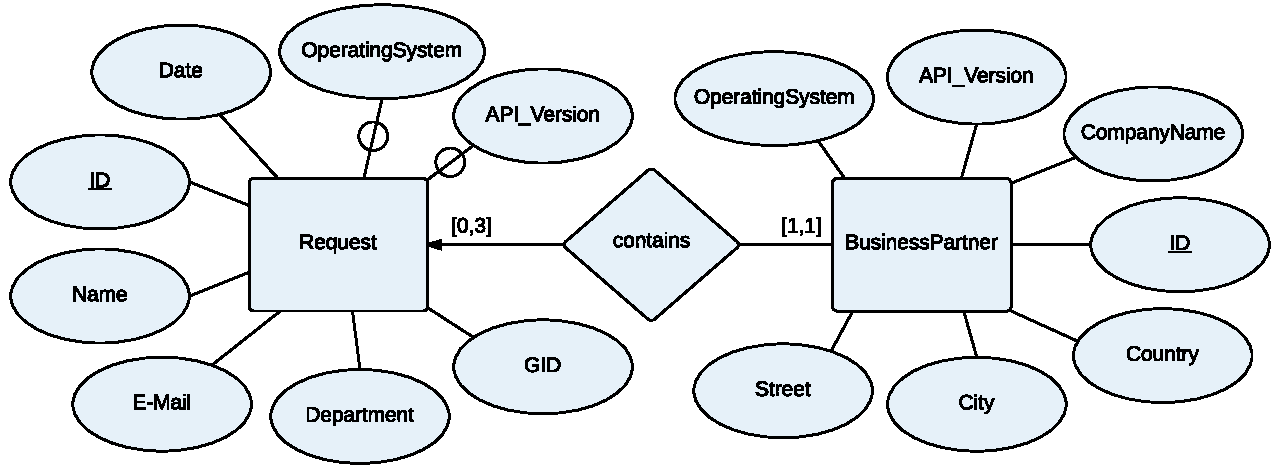
\includegraphics[width=0.8\textwidth]{\figdir/er-model.pdf}
\end{figure}

Ut wisi enim ad minim veniam, quis nostrud exerci tation ullamcorper suscipit lobortis nisl ut aliquip ex ea commodo consequat. Duis autem vel eum iriure dolor in hendrerit in vulputate velit esse molestie consequat, vel illum dolore eu feugiat nulla facilisis at vero eros et accumsan et iusto odio dignissim qui blandit praesent luptatum zzril delenit augue duis dolore te feugait nulla facilisi

\section{PouchDB}
\label{sec:Szenarien}
\begin{citeenv}
  \begin{quotation}
    "`Und hier als Einstieg ein tolles Zitat."' \cite{book:eckert}.
  \end{quotation}
\end{citeenv}

Es folgt eine \emph{hervorgehobener Text}. Akronyme -- wie zum Beispiel \acr{BLAUNDBLUB} können natürlich auch komfortabel eingepflegt werden. Eine Fußnote\footnote{"`[\ldots] a protocol useful in determining the current status of a digital certificate without requiring Certificate Revocation Lists"' \cite{tech:rfc6960}.} wird mit backslash footnote eingefügt.

Lorem ipsum dolor sit amet, consetetur sadipscing elitr, sed diam nonumy eirmod tempor invidunt ut labore et dolore magna aliquyam erat, sed diam voluptua. At vero eos et accusam et justo duo dolores et ea rebum. Stet clita kasd gubergren, no sea takimata sanctus est Lorem ipsum dolor sit amet.

\paragraph{Erster Absatz}
\label{par:Usecase 1}
Lorem ipsum dolor sit amet, consetetur sadipscing elitr, sed diam nonumy eirmod tempor invidunt ut labore et dolore magna aliquyam erat, sed diam voluptua. At vero eos et accusam et justo duo dolores et ea rebum. Stet clita kasd gubergren, no sea takimata sanctus est Lorem ipsum dolor sit amet.

\paragraph{Zweiter Absatz}
\label{par:Usecase 2}
Lorem ipsum dolor sit amet, consetetur sadipscing elitr, sed diam nonumy eirmod tempor invidunt ut labore et dolore magna aliquyam erat, sed diam voluptua. At vero eos et accusam et justo duo dolores et ea rebum. Stet clita kasd gubergren, no sea takimata sanctus est Lorem ipsum dolor sit amet. Lorem ipsum dolor sit amet, consetetur sadipscing elitr, sed diam

\chapter{Verwendeter Technologiestack}
\label{chap:Technologien}
Wisi enim ad minim veniam, quis nostrud exerci tation ullamcorper suscipit lobortis nisl ut aliquip ex ea commodo consequat.

\section{Erste tolle Technologie, auf die eingegangen wird}
\label{sec:Erste Technologie}

\marginnote{Marginnote} Marginnotes habe ich in meiner BA verwendet. Brauchen wir wahrscheinlich nicht unbedingt.

Duis autem vel eum iriure dolor in hendrerit in vulputate velit esse molestie consequat, vel illum dolore eu feugiat nulla facilisis at vero eros et accumsan et iusto odio dignissim qui blandit praesent luptatum zzril delenit augue duis dolore te feugait nulla facilisi. Lorem ipsum dolor sit amet, consectetuer adipiscing elit, sed diam nonummy nibh euismod tincidunt ut laoreet dolore magna aliquam erat volutpat.

\marginnote{Schlagwort}
Ut wisi enim ad minim veniam, quis nostrud exerci tation ullamcorper suscipit lobortis nisl ut aliquip ex ea commodo consequat. Duis autem vel eum iriure dolor in hendrerit in vulputate velit esse molestie consequat, vel illum dolore eu feugiat nulla facilisis at vero eros et accumsan et iusto odio dignissim qui blandit praesent luptatum zzril delenit augue duis dolore te feugait nulla facilisi.

Und noch ein fetter \textbf{Text} und eine Tabelle, die auch über mehrere Seiten gehen darf:

\renewcommand{\arraystretch}{2}
 \begin{center}
   \begin{longtable}{| C{0.08\twfivec} | L{0.2\twfivec} | p{0.48\twfivec} | C{0.1\twfivec} | C{0.14\twfivec} |} % longtable kann über mehrere Seiten umbrechen, alternativ kann tabularx verwendet werden, die die Breite automatisch berechnet.
     \caption{Beispieltabelle}\label{t:Beispieltabelle}\\
     \hline
     \textbf{ID} & \textbf{Name} & \textbf{Beschreibung} & \textbf{Prio} & \textbf{Abhängig} \\
     \hline
     \hline
     \endfirsthead
     \multicolumn{5}{l}%
     {\tablename\ \thetable\ -- \textit{Fortsetzung von vorheriger Seite}} \\
     \hline
     \textbf{ID} & \textbf{Name} & \textbf{Beschreibung} & \textbf{Prio} & \textbf{Abhängig} \\
     \hline
     \hline
     \endhead
     \hline \multicolumn{5}{r}{\textit{Fortsetzung auf nächster Seite}} \\
     \endfoot
     \endlastfoot
      /01/ & Antragsteller Daten & Wisi enim ad minim veniam, quis nostrud exerci tation ullamcorper suscipit lobortis nisl ut aliquip ex ea commodo consequat. & Should & - \\
      \hline
      /02/ & Eigenbedarf oder GP & Wisi enim ad minim veniam, quis nostrud exerci tation ullamcorper suscipit lobortis nisl ut aliquip ex ea commodo consequat. & Must & - \\
      \hline
      /03/ & Daten Geschäftspartner & Wisi enim ad minim veniam, quis nostrud exerci tation ullamcorper suscipit lobortis nisl ut aliquip ex ea commodo consequat. & Must & - \\
      \hline
      /04/ & \hspace{0pt}Mehrfachangabe & Wisi enim ad minim veniam, quis nostrud exerci tation ullamcorper suscipit lobortis nisl ut aliquip ex ea commodo consequat. & Should & - \\
      \hline
      /05/ & \hspace{0pt}Betriebssystem & Wisi enim ad minim veniam, quis nostrud exerci tation ullamcorper suscipit lobortis nisl ut aliquip ex ea commodo consequat. & Must & - \\
      \hline
      /016 & Lizenz-Bestimmungen &  Wisi enim ad minim veniam, quis nostrud exerci tation ullamcorper suscipit lobortis nisl ut aliquip ex ea commodo consequat. & Must & - \\
      \hline
      /07/ & Datum & Wisi enim ad minim veniam, quis nostrud exerci tation ullamcorper suscipit lobortis nisl ut aliquip ex ea commodo consequat. & Must & - \\
      \hline
  \end{longtable}
\end{center}


Eine Formel:
\begin{equation}
\label{eq:kardinalität}
contains(Request[0,3], BusinessPartner[1,1])
\end{equation}

Eine Aufzählung in Latex schaut dann so aus:
\begin{itemize}
  \item Erster Punkt
  \item Zweiter schlauer Punkt
  \item Dritter vielleicht noch schlauerer Punkt
\end{itemize}

Eine Grafik, die in zwei Teile aufgeteilt ist:

\begin{figure}[ht]
\centering
\begin{subfigure}{\textwidth}
\caption{Graphik erster Teil}
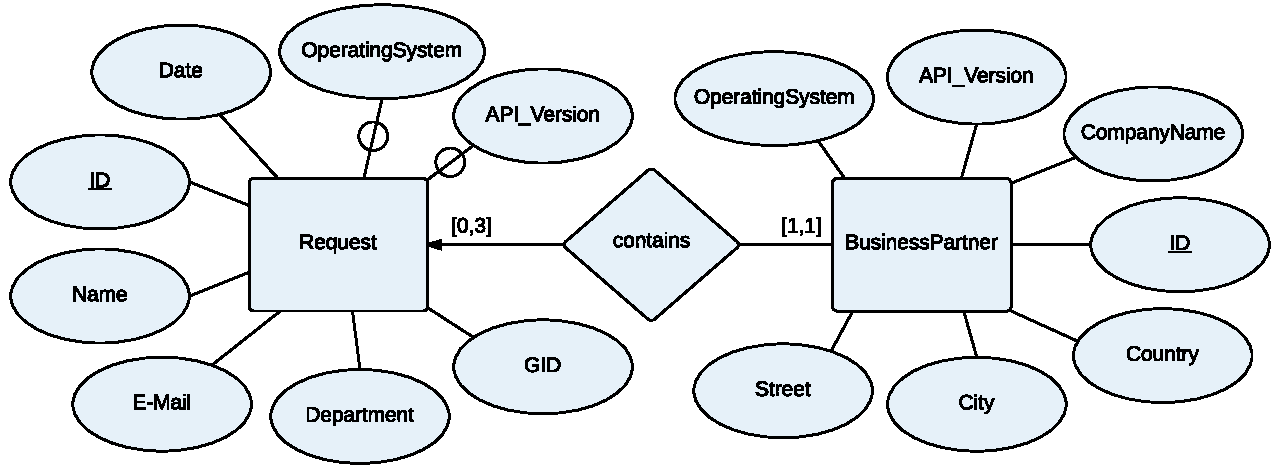
\includegraphics[width=\textwidth]{\figdir/er-model.pdf}
\end{subfigure}
\end{figure}

\begin{figure}[H]
\ContinuedFloat
\centering
\begin{subfigure}{\textwidth}
\caption{Zweiter Teil}
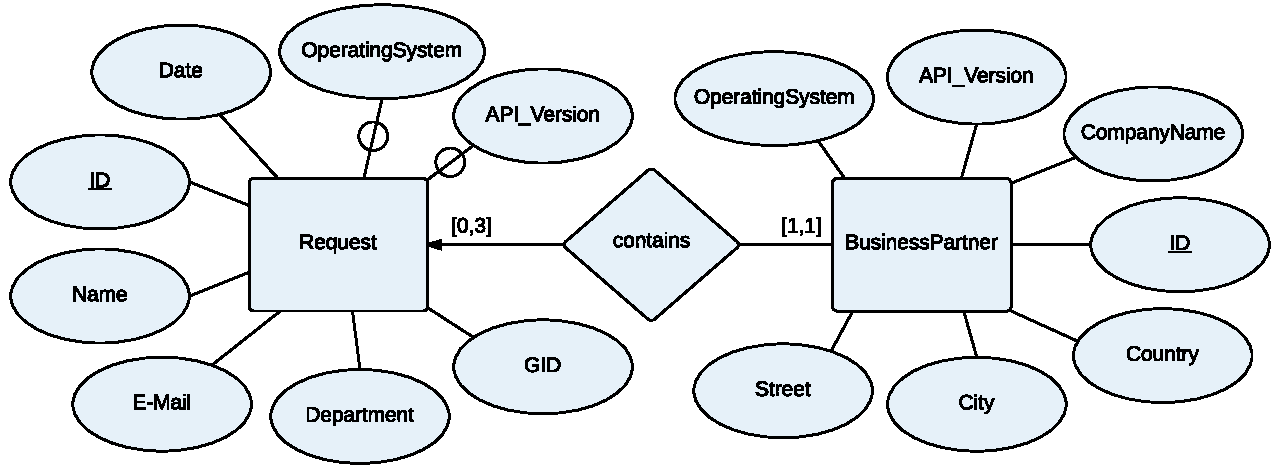
\includegraphics[width=\textwidth]{\figdir/er-model.pdf}
\end{subfigure}
\caption{Nochmal die gleiche Beispielgrafik}
\label{fig:workflow}
\end{figure}

So und jetzt viel Spaß mit \LaTeX!! Am anfang muss man zwar viel googlen, aber geht eigentlich relativ schnell. Könnt mich auch gerne fragen wenn irgendwas unklar ist.

%\input{./chapters/blub2}
%\input{./chapters/blub3}

\cleardoublepage

% \bibliographystyle{natger} %für backend biber
% \bibliography{thesis} %für backend biber
\printbibliography

\cleardoublepage


\footnotesize
\printindex


\end{document}
